\setchapterimage[6cm]{chapter/aircraft/aircraft_title_photo2.jpg}
\setchapterpreamble[u]{\margintoc}
\chapter[Aircraft and their manufacturers]{Aircraft and their manufacturers\protect\footnotemark}
\labch{aircraft-chapter_en}

\footnotetext{\href{https://en.wikipedia.org/wiki/NASA_X-43}{NASA X-43} it is the fastest aircraft in the history of aviation.
Author: \href{https://commons.wikimedia.org/wiki/File:X43a2_nasa_scramjet.jpg}{NASA, WikiCommons / 2008 / Public Domain}. }

The chapter explores the various properties of aircraft based on the Wikidata database.
During the study, using SPARQL queries calculated on objects of the ``Aircraft'' type, a list of aircraft and their manufacturers was obtained, the number 
produced aircraft for different models. For this number of aircraft, the \Wikiref{Pareto principle} has been verified by models.
A diagram is also obtained showing the ratio of the total number of aircraft manufacturers by country.
The chapter concludes with an estimate of the completeness of the data presented in Wikipedia and Wikidata. 
According to it, only 595 records of aircraft manufacturers from \num{1700} for 2020 are presented in Wikidata.
Assuming a fixed number of new aircraft manufacturers emerge each year and the number of Wikidata entries entered annually, 
we can assume that in about 75 years (that is, in 2095) Wikidata will contain records of all aircraft manufacturers.


%%%%%%%%%%%%%%%%%%%%%%%%%%%%%%%%%%%%%%%%%%%%%%%%%%%%%%%

\section{List of aircrafts}

Aircraft~--- an aircraft supported in the atmosphere by interaction with air, different from interaction with air reflected from the 
surface of the earth or water.
Aircraft include the following types of aircraft: gyroplane, balloon, helicopter, rotorcraft, airship, flywheel, glider and airplane.
Aircraft do not include spaceships, rockets, ekranoplanes (but not ekranoplanes) and hovercraft.

Let's build a list of all instances of the object ``Aircraft'' \href{https://www.wikidata.org/wiki/Q11436}{Q11436}.

\begin{lstlisting}[ language=SPARQL, breaklines=true, 
                    caption={List of aircrafts.\\\hspace{\textwidth}
                        The result contains \num{1564} aircrafts in 2017, 
                        \num{3324} aircrafts in 2020.\\\hspace{\textwidth}
                        SPARQL query: \href{https://w.wiki/rez}{w.wiki/rez}
                        },
                    label=lst:aircraft_listing_1,
                    texcl 
                    ]
# List of aircrafts
SELECT ?plane ?planeLabel
WHERE
{
    ?plane wdt:P31 wd:Q11436. # instance of aircraft
    SERVICE wikibase:label {bd:serviceParam wikibase:language "en"}
}
\end{lstlisting}

The most complete and well-developed aircraft on Wikidata in 2017 were \href{https://www.wikidata.org/wiki/Q271446}{Mikoyan-Gurevich MiG-3}, 
\href{https://www.wikidata.org/wiki/Q1349098}{Yakovlev Yak-36}, \href{https://www.wikidata.org/wiki/Q429839}{Mitsubishi A5M}. 
As for 2020, the most complete and well-developed aircrafts on Wikidata are \href{https://www.wikidata.org/wiki/Q770863}{Sopwith Triplane} (18 properties), 
\href{https://www.wikidata.org/wiki/Q1658673}{IL-103} (14 properties), \href{https://www.wikidata.org/wiki/Q665071}{Martin 2-0-2} (14 properties).
%Almost empty and uninformative aircraft for 2017 turned out to be: \href{https://www.wikidata.org/wiki/Q464247}{Mikoyan-Gurevich MiG-1}, 
%\href{https://www.wikidata.org/wiki/Q2296502}{Sukhoi Su-6}, \href{https://www.wikidata.org/wiki/Q1658673}{Il-103}.
For 2020, uninformative aircraft are: \href{https://www.wikidata.org/wiki/Q820603}{Beriev Be-1} (Wikidata object has 3 properties), \href{https://www.wikidata.org/wiki/Q117984}{Lituanica} (Wikidata object has 4 properties), 
\href{https://www.wikidata.org/wiki/Q572762}{Lavochkin La-168} (Wikidata object has 3 properties).

%%%%%%%%%%%%%%%%%%%%%%%%%%%%%%%%%%%%%%%%%%%%%%%%%%%%%%%

\section{Aircraft manufacturers}

Let's make a list of aircraft manufacturers by completing the request~\ref{lst:aircraft_listing_2}.

\index{SPARQL!COUNT!Aircraft manufacturers}
\begin{lstlisting}[ language=SPARQL, breaklines=true, 
                    caption={Aircraft manufacturers\\\hspace{\textwidth}
                        The result contains \num{300} manufacturers in 2017, 
                        \num{597} manufacturers in 2020.\\\hspace{\textwidth}
                        SPARQL query: \href{https://w.wiki/vNn}{w.wiki/vNn}
                        },
                    label=lst:aircraft_listing_2,
                    texcl 
                    ]
# Count aircraft having property manufacture, group by manufacture
SELECT ?manufacture ?manufactureLabel (COUNT(?plane) AS ?count) 
WHERE {
  ?plane wdt:P31 wd:Q11436. # instance of aircraft
  ?plane wdt:P176 ?manufacture. # show manufacture
  SERVICE wikibase:label {bd:serviceParam wikibase:language "en".}
}
GROUP BY ?manufacture ?manufactureLabel
\end{lstlisting}

The result of the query~\ref{lst:aircraft_listing_2} is a list of all aircraft manufacturers.

%%%%%%%%%%%%%%%%%%%%%%%%%%%%%%%%%%%%%%%%%%%%%%%%%%%%%%%

\label{question:aircraft_manufacturers_en}
\marginnote{
Which of the Russian aircraft manufacturers below have websites?
\begin{itemize}
\item \Wikiref{Russian Aircraft Corporation MiG}
\item \Wikiref{Saratov Aviation Plant}
\item \Wikiref{Tupolev}
\item \Wikiref{Sukhoi}
\end{itemize}
The answer is on page~\pageref{answer:aircraft_manufacturers_en}.
}


\section{Number of aircraft produced}

\index{Aircraft!Aviation industry!definition}
The aviation industry is one of the largest mechanical engineering industries in the world. Its tasks include both the development 
and production of various aerial vehicles. In order to assess which aircraft models are the most widespread, we will build a diagram 
of the produced aircraft of various models, , shown in Fig.~\ref{fig:Number_of_aircraft_produced_en_2020}.
To get the number of aircraft produced, query~\ref{lst:aircraft_listing_3}.


\begin{lstlisting}[ language=SPARQL, breaklines=true, 
                    caption={Received \num{288} models, for which the number\\\hspace{\textwidth}
                        of aircraft produced, 2020 is known. 
                        SPARQL query: \href{https://w.wiki/v4J}{w.wiki/v4J}
                        },
                    label=lst:aircraft_listing_3,
                    texcl 
                    ]
# List of aircraft models, sorted by number of aircraft built
SELECT ?plane ?planeLabel ?planes_produced WHERE {
  ?plane wdt:P31 wd:Q11436. # instance of aircraft
  ?plane wdt:P1092 ?planes_produced.  # total aircraft manufactured
  SERVICE wikibase:label {bd:serviceParam wikibase:language "ru,en".}
}
ORDER BY DESC(?planes_produced)
\end{lstlisting}

Some aircraft models were produced in small numbers, so they can be excluded to improve the readability of the diagram~\ref{fig:Number_of_aircraft_produced_en_2020}. 
To get a new list, let's add a filter to the request~\ref{lst:aircraft_listing_4}.

\index{SPARQL!FILTER!List of aircraft manufactured over 10 pieces}
\begin{lstlisting}[ language=SPARQL, breaklines=true, 
                    caption={A list of \num{124} models, filtered by the\\\hspace{\textwidth}
                        number of aircraft produced, has been received.
                        SPARQL query: \href{https://w.wiki/v4N}{w.wiki/v4N}
                        },
                    label=lst:aircraft_listing_4,
                    texcl 
                    ]
# List of aircraft models, sorted by number of aircraft built
#defaultView:BarChart
SELECT ?plane ?planeLabel ?planes_produced WHERE {
  ?plane wdt:P31 wd:Q11436. # instance of aircraft
  ?plane wdt:P1092 ?planes_produced.  # total aircraft manufactured
  FILTER (?planes_produced > 10)
  SERVICE wikibase:label {bd:serviceParam wikibase:language "ru,en".}
}
ORDER BY (?planes_produced)
\end{lstlisting}

The figure in Fig.~\ref{fig:Number_of_aircraft_produced_en_2020} shows that the following aircraft models were produced the most in 
2020: \href{https://www.wikidata.org/wiki/Q2096452}{PA-32 Cherokee Six} (\num{7842} pieces), \href{https://www.wikidata.org/wiki/Q1860367}{Piper PA-24 Comanche} 
(\num{4857}), \href{https://www.wikidata.org/wiki/Q694521}{Junkers W 34} (\num{3000}), \href{https://www.wikidata.org/wiki/Q941011}{Pomilio PE} 
(\num{1616}).

\begin{figure*}[h]

    \setlength{\fboxsep}{0pt}%
    \setlength{\fboxrule}{1pt}%
    \fcolorbox{gray}{gray}{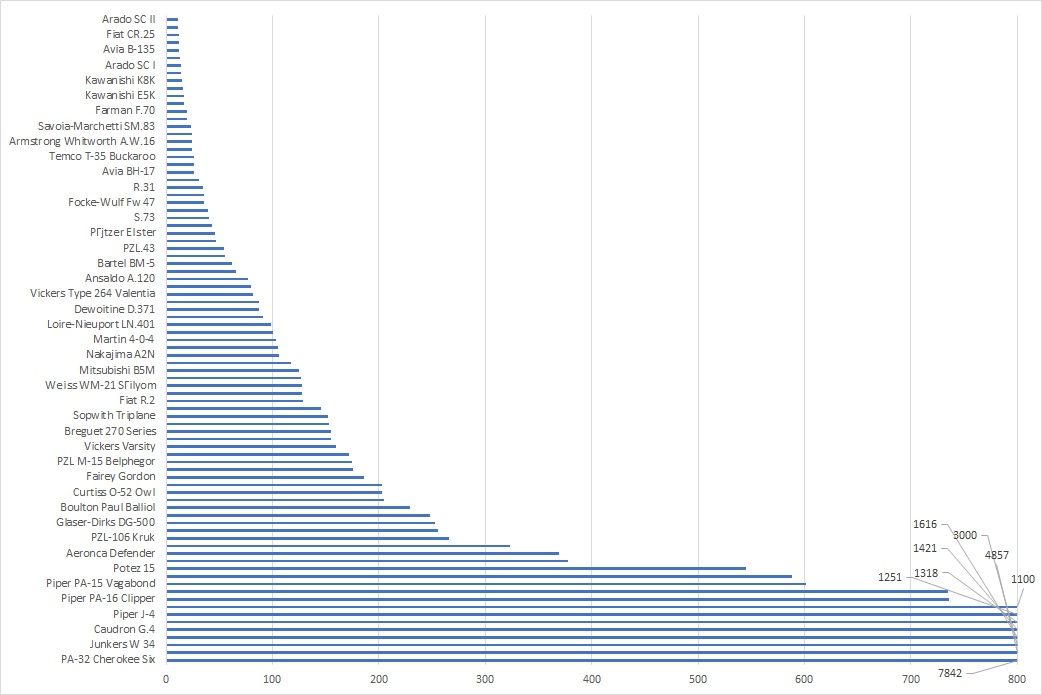
\includegraphics[width=\linewidth]{./chapter/aircraft/Number_of_aircraft_produced_en_2020.jpg}}%

	\caption[Number of aircraft produced by model, 2020.]{The number of aircraft produced by model, 2020. The diagram is built in Microsoft Excel based on the data obtained using the query ~\protect\ref{lst:aircraft_listing_4}.}%
    \label{fig:Number_of_aircraft_produced_en_2020}%
\end{figure*}

Now let's try to answer the question: ``Does \Wikiref{Pareto principle} hold with respect to the 
number of aircraft models''?

In order to build a graph, you must perform the following steps:

\begin{enumerate} 
  \item Calculate the total number of aircraft for all models using the script shown in the listing~\ref{lst:aircraft_listing_5}.

  \index{SPARQL!SUM / Total number of aircraft produced}
  \begin{lstlisting}[ language=SPARQL, breaklines=true,  
                      caption={Total number of aircraft produced\\\hspace{\textwidth}
                          The result contains \num{33 178} aircrafts in 2020.
                          SPARQL query: \href{https://w.wiki/rf9}{w.wiki/rf9}
                          },
                      label=lst:aircraft_listing_5,
                      texcl 
                      ]
  SELECT (SUM(?count) as ?sum) WHERE {
    SELECT ?count WHERE {
      SERVICE wikibase:label {bd:serviceParam wikibase:language "en".}
      ?plane wdt:P31 wd:Q11436; # instance of aircraft
			 wdt:P1092 ?count. # total aircraft manufactured
    }
  }
  \end{lstlisting}
  
  \label{question:aircraft_question_2}
  \marginnote{
	Find the correspondence between the date of foundation and the company in the following table:
	\\
	\begin{tabular}{ l | l }
	Company & Foundation date \\ \hline
	\Wikiref{MiG} & January 1, 1939 \\
	\Wikiref{Vympel NPO} & November 18, 1949 \\
	\Wikiref{Tupolev} & December 18, 1939 \\
	\Wikiref{Sukhoi} & January 1, 1922 \\
	\end{tabular}
	\\
	The answer is on page~\pageref{answer:aircraft_answer_2}.
  }
  
  \item The X axis represents the number of aircraft models under consideration (that is, for x = 1, we consider the number of aircraft of the first model 
  produced, for x = 2~--- the number of aircraft of the first and second model, and so on). 
  On the Y axis we will plot F(n) = $\sum\limits_{i=1}^n f(i)$, where f(i)~--- is the number of aircraft of model i released. 
  In this case, the condition f(i) > f(j) is satisfied, for i < j, where i, j~--- is the aircraft model number 
  (that is, the number of released aircraft models is pre-ordered in descending order). Also, on the X-axis, we postpone the second scale from 0 to 1, 
  to make it easier to determine the parameters for checking the implementation of \Wikiref{Pareto principle}.
  
\end{enumerate}



\begin{figure*}[h]

    \setlength{\fboxsep}{0pt}%
    \setlength{\fboxrule}{1pt}%
    \fcolorbox{gray}{gray}{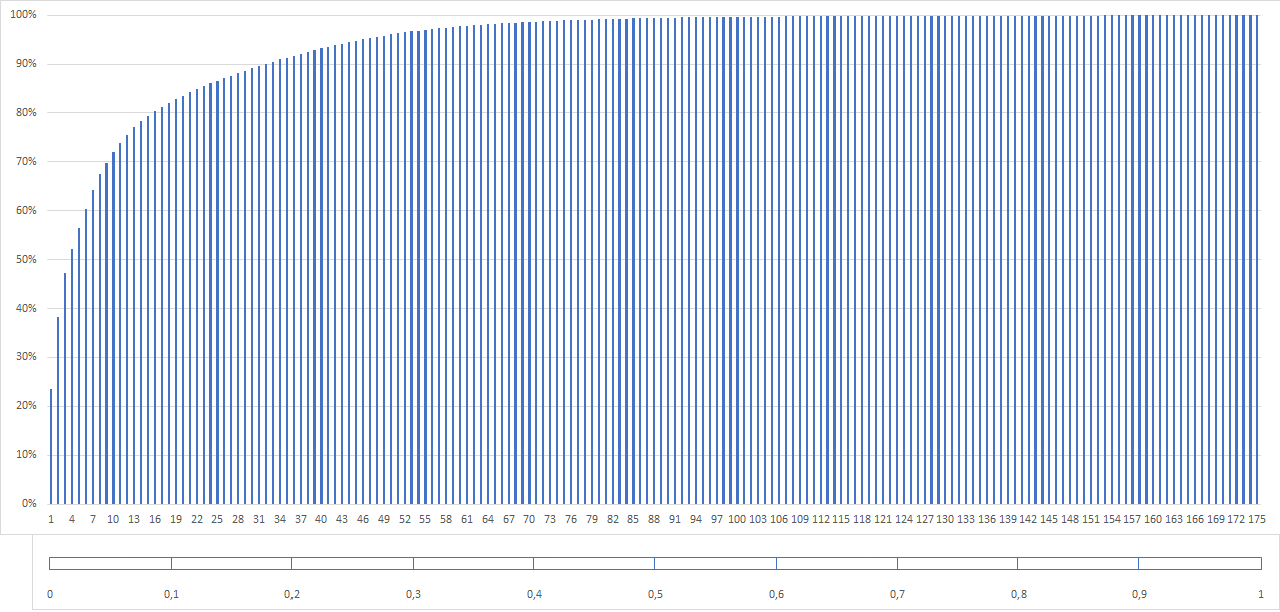
\includegraphics[width=\linewidth]{./chapter/aircraft/Pareto_principle_diargam_en.png}}%

%	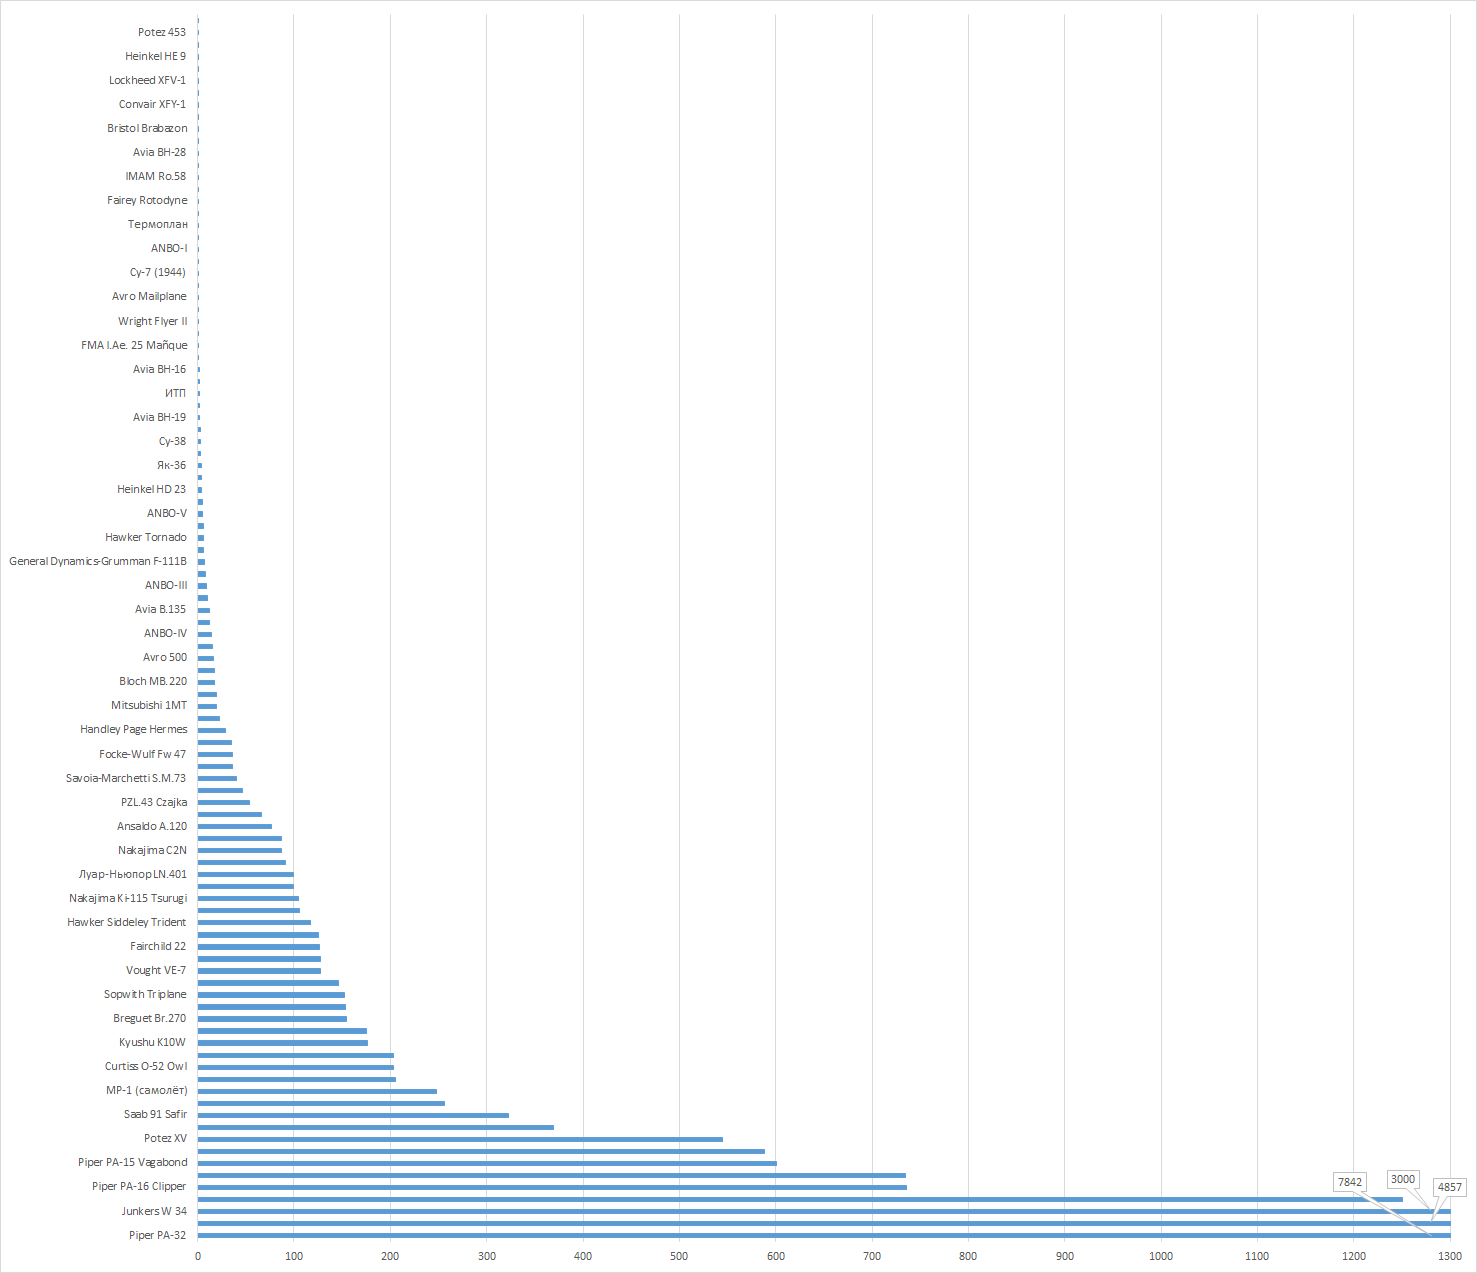
\includegraphics{chapter/aircraft/Number_of_aircraft_produced_ru.png}%
	\caption{Percentage of the number of aircraft models produced by all airlines to the total number of aircraft manufactured for all time, 2020.}%
    \label{fig:Pareto_principle_diargam_en}%
\end{figure*}

According to the graph~\ref{fig:Pareto_principle_diargam_en}, it can be seen that 80\% of all aircraft produced belong to 16 different aircraft 
models, which is 9.2\% of the total number of models. Pareto's law states that: ``20\% of the efforts give 80\% of the result, and the remaining 80\%
 of the efforts~--- only 20\% of the result''. It can be concluded that a stronger law is fulfilled than the Pareto principle regarding the number 
 of aircraft models.

\label{question:aircraft_question_3}
\marginnote{
Find the correspondence between the location of the company's headquarters and the company.
\\
\begin{tabular}{ l | l }
Company & Headquarters \\ \hline
\Wikiref{Kazan Helicopters} & Kazan \\
\Wikiref{Saratov Aviation Plant} & Saratov \\
\Wikiref{Ulan-Ude Aviation Plant} & Ulan-Ude \\
\Wikiref{Sukhoi} & Moscow \\
\end{tabular}
\\
The answer is on page~\pageref{answer:aircraft_company_headquarters_en}.
}

%%%%%%%%%%%%%%%%%%%%%%%%%%%%%%%%%%%%%%%%%%%%%%%%%%%%%%%

\section{In which countries are aircraft produced}

Let's build a list of the number of aircraft manufacturers by country. To execute the query~\ref{lst:aircraft_listing_7}, we use the grouping 
by country (GROUP BY) and use the ``Count'' function for each country to calculate the total number of aircraft manufacturing plants.

%\index{SPARQL!COUNT!List of the ratio of the number of manufacturers aircraft by country}
%\begin{lstlisting}[ language=SPARQL, breaklines=true, 
%                    caption={List of the ratio of the \\\hspace{\textwidth} 
%						number of manufacturers aircraft by country\\\hspace{\textwidth}
%                        The result contains \num{39} records in 2017, 
%                        \num{46} records in 2020.\\\hspace{\textwidth}
%                        SPARQL query: \href{https://w.wiki/rfD}{w.wiki/rfD}
%                        },
%                    label=lst:aircraft_listing_6,
%                    texcl 
%                    ]
%# Count manufacture having property country group by country
%SELECT ?countryLabel (count(?manufacture) as ?count)
%WHERE
%{
%    ?manufacture wdt:P31 wd:Q936518. # instance of aerospace manufacture
%  	?manufacture wdt:P17 ?country. # belong to country
%    SERVICE wikibase:label { bd:serviceParam wikibase:language "en" }
%}
%GROUP BY ?country ?countryLabel
%\end{lstlisting}

Having received a list of countries by the number of aircraft manufacturing plants, we can construct a bubble diagram 
for clarity of the ``Relationship between the number of aircraft manufacturers by country''~\ref{fig:Manufacture-with-country_2020_en}. 
To build it, we execute the request ~\ref{lst:aircraft_listing_7}.

\index{SPARQL!COUNT!Bubble chart ``Relationship between the number of aircraft manufacturers by country''}
\index{Chart!BubbleChart!Bubble chart ``Relationship between the number of aircraft manufacturers by country''}
\begin{lstlisting}[ language=SPARQL, breaklines=true, 
                    caption={Bubble chart\\\hspace{\textwidth}
                        SPARQL query: \href{https://w.wiki/vPE}{w.wiki/vPE}
                        },
                    label=lst:aircraft_listing_7,
                    texcl 
                    ]
#defaultView:BubbleChart
SELECT ?country ?countryLabel (count(?manufacture) as ?count)
WHERE
{
    ?manufacture wdt:P31 wd:Q936518. # instance of aerospace manufacture
  	?manufacture wdt:P17 ?country. # belong to country
    SERVICE wikibase:label {bd:serviceParam wikibase:language "en"}
}
GROUP BY ?country ?countryLabel
\end{lstlisting}

The query~\ref{lst:aircraft_listing_7} will generate a bubble chart in which the circles represent countries and their sizes correspond to the number 
of aircraft manufacturers in the specified country. Such a diagram helps to more clearly see the difference in the number of aircraft factories 
between countries.

\begin{figure}[h!]
\centering
	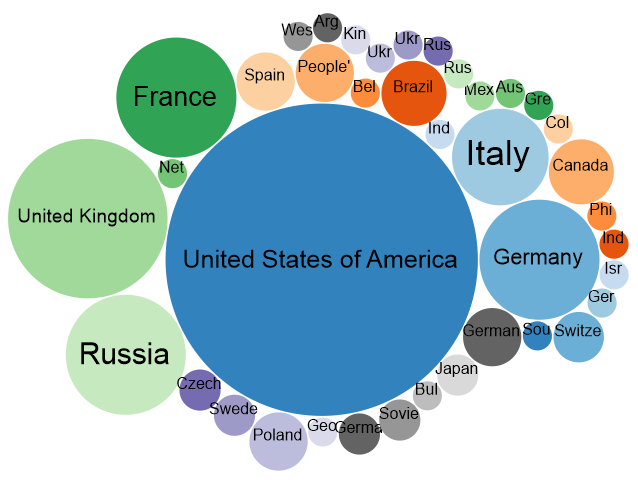
\includegraphics[width=0.95\textwidth]{./chapter/aircraft/Manufacture-with-country_en_2017.png}
	\caption{The ratio of the number of aircraft manufacturers by country, 2017.}
	\label{fig:Manufacture-with-country_en_2017}
\end{figure}

As can be seen from the response to request~\ref{lst:aircraft_listing_7} in Fig.~\ref{fig:Manufacture-with-country_en_2017}, not all existing 
aircraft manufacturers are listed, as evidenced by the data taken from the \href{https://www.aviationfanatic.com/}{aviationfanatic.com}. 
More information about the lack of data in Wikidata is given in the next section of this chapter. 
%Most manufacturers are indicated in the USA (115), Great Britain (30), Germany (17), Russia (17) as of May 2017.

\label{question:aircraft_question_4}
\marginnote{
What is the name of an aircraft held in the air by a huge tank of flammable, lethal gas, located directly above the heads of passengers?
\\
The answer is on page~\pageref{answer:aircraft_question_airship_en}.
}


\begin{figure}[h!]
\centering
	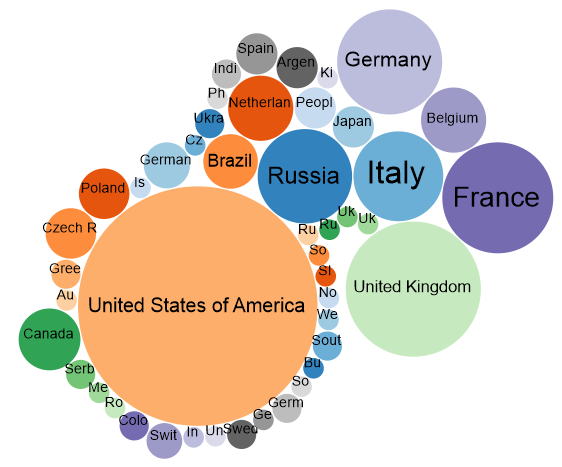
\includegraphics[width=0.95\textwidth]{./chapter/aircraft/Manufacture-with-country_2020_en.png}
	\caption{The ratio of the number of aircraft manufacturers by country, 2020.}
	\label{fig:Manufacture-with-country_2020_en}
\end{figure}


Comparing two bubble charts for 2017 (Fig.~\ref{fig:Manufacture-with-country_en_2017}) and 2020 (Fig.~\ref{fig:Manufacture-with-country_2020_en}), 
we can conclude that the main aircraft manufacturers in the world in 2017 and 2020 were: USA (115 plants in 2017 and 135 plants in 2020), 
Great Britain (30 and 43 plants), Germany (17 and 26 plants) and Russia (17 and 21 plants). The USA is still the leader, but France in 3 years 
managed to outstrip Germany, increasing the number of production facilities to 29 (Germany~--- 26), thus taking the third place. But in general, 
the ratio of aircraft production between different countries remains the same.

%%%%%%%%%%%%%%%%%%%%%%%%%%%%%%%%%%%%%%%%%%%%%%%%%%%%%%%

\section{Completeness of Wikidata}


\label{question:aircraft_question_5}
\marginnote{
Which aircraft is shown in Fig.~\ref{fig:airship-SSSR-V6-uknown}?
}


\begin{marginfigure}
{
\setlength{\fboxsep}{0pt}%
\setlength{\fboxrule}{1pt}%
\fcolorbox{gray}{gray}{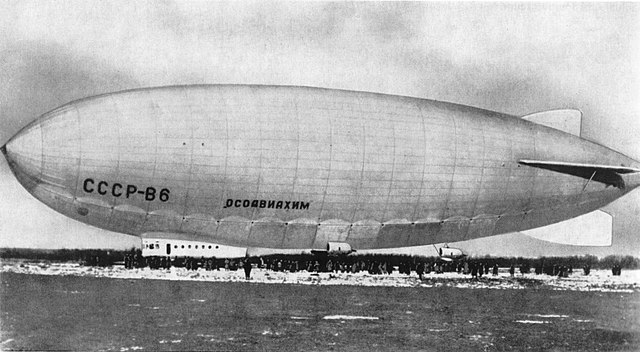
\includegraphics[width=\linewidth]{./chapter/aircraft/airship-SSSR-V6.jpg}}%
}
  \caption{Unknown aircraft.}%
  \label{fig:airship-SSSR-V6-uknown}%
\end{marginfigure}


\marginnote{
The answer is on page~\pageref{answer:aircraft_question_airship_2_en}.
}


Based on the above data, it is possible to predict when Wikidata will include all data from aviationfanatic.com. In three years, 
the number of aircraft manufacturers increased by 239, representing an annual increase of about 80 aircraft manufacturers. 
Also during this time, information on 295 aircraft manufacturers was entered into Wikidata, that is, about a hundred aircraft factories 
are added annually. For 2020, there was no information on Wikidata about the \num{1344} aircraft manufacturers listed 
on \href{https://www.aviationfanatic.com/}{aviationfanatic.com}. Assuming that a fixed number of new aircraft manufacturers are added 
annually and the number of entries in Wikidata remains unchanged, we can assume that in about 75 years (i.e. 2095), Wikidata will contain 
records of all aircraft manufacturers listed on the aviationfanatic website. com.

The category \Wikiref{Category:Aircraft manufacturers of Russia} indicates the presence in Russia of 58 aircraft manufacturing companies 
in 2017 and 62 plants, institutes and corporations related to aircraft manufacturing in 2020, but at the same time on the 
website \href{https://www.aviationfanatic.com/}{Aviationfanatic.com} lists 61 plants in 2017 and 71 in 2020. 
Among the aircraft building companies in Russia are such companies as: \Wikiref{Irkut Corporation}, \Wikiref{MiG}, \Wikiref{Tupolev}.

%%%%%%%%%%%%%%%%%%%%%%%%%%%%%%%%%%%%%%%%%%%%%%%%%%%%%%%

\section{Exercises}
 
\begin{enumerate}
\item Find the plane with the maximum flight radius.
\item Mark on the political map of the world the location of the main offices of aircraft manufacturers.
\item Find the manufacturer with the maximum number of aircraft manufactured using the \href{https://w.wiki/vF7}{\textit{manufacturer (P176)}} property for aircraft.
\item When was the first aircraft built?
\item Which firms were the first to produce 10, 100 and a thousand aircraft?
\item Draw a chart of the number of aircraft produced in the world and in Russia by year.
\end{enumerate}
